\section{Experiments} \label{c:experiments}

%
This section contains results of experiments that were performed on the multiset-trie 
data structure. In particular, we will test the functions: \textsc{submsetExistence}, 
\textsc{supermsetExistence}, \textsc{getAllSubmsets} and 
\textsc{getAllSupermsets}. 

The implementation of multiset-trie is done in the \CC 
{ programming} language. The current implementation uses only the standard 
library of \CC14 version of the standard and has a command line interface. The implementation 
of the program was optimized for testing and therefore, the program operates 
with files, in order to process queries. After processing all the queries 
the results are stored in files for further analysis.

%Performance of the functions will be measured by 
%the number of visited nodes in multiset-trie by the particular function. In 
%particular the performance is inversely proportional to the number of visited 
%nodes.

Before we start, we will give a few definitions about the parameters 
that will be varied throughout the experiments and discuss the experimental data 
that was used.

Let $M$ be a set of multisets that are inserted to multiset-trie and let $n$ be 
the maximal node degree. Let $N$ be the power multiset of $\Sigma,$ where 
the multiplicity of each element is bounded from above by $n-1.$ We define the 
\emph{density} of a multiset-trie to be the ratio $\frac{|M|}{|N|},$ where 
$|\cdot|$ denotes cardinality.

The selected parameters of the data structure that will be varied in experiments 
are as follows:
%
\begin{itemize}
\item $\sigma$ - the cardinality of the alphabet $\Sigma;$
%
\item $n$ - the maximal degree of a node, which explicitly defines the maximal 
multiplicity of elements in a multiset;
%
\item $\phi$ - mapping of letters from $\Sigma$ into a set of consecutive 
integers;
%
\item $d$ - density of a multiset-trie.
%
\end{itemize}
The cardinality of a power multiset $N$ is equal to $n^\sigma,$ which means that 
density $d$ of a multiset-trie depends on parameters $|M|,$ $\sigma$ and $n.$ 
Because parameters $\sigma$ and $n$ are set when a multiset-trie is initialized, 
the parameter $|M|$ will be varied to change the density in experiments. As we 
mentioned in Section~\ref{c:description}, the mapping $\phi$ determines the 
correspondence of letters to levels in multiset-trie, i.e. it defines the ordering of 
levels in multiset-trie. It is also true, that $\phi$ defines the ordering in multisets.

% anouncement of the experiments
In the next sections we will present the behavior of the multiset-trie data 
structure depending on the selected parameters as well as the comparative 
benchmark of the multiset-trie against B+ tree implementation of inverted index. 
% outline of the experiment section
We start with experiments that are performed on an artificially generated data in 
order to give a general picture of the multiset-trie performance. In the 
Experiment~\hyperref[s:exp1]{1} a special case of the multiset-trie is considered. 
Only sets are allowed to be stored in the data structure, i.e. the maximal allowed 
multiplicity is set to 1. The performance is measured with respect to the density 
of the multiset-trie.
%
The Experiment~\hyperref[s:exp2]{2} is an extension of the previous one. Here, 
we also measure the performance of the multiset-trie depending on its density. 
The difference is that the allowed multiplicity of an element is raised, i.e. 
the data structure is populated with multisets. 
%
Summarizing the tests of performance depending on the density we present the 
Experiment~\hyperref[s:exp3]{3}. It shows a non linearity of the performance 
with respect to the density of the multiset-trie.
%
The next experiment on the multiset-trie uses the real world data. In 
Experiment~\hyperref[s:exp4]{4} the influence of the mapping $\phi$ is studied. 
The input data is obtained by mapping of the real words from English dictionary 
to the set of consecutive integers using the function $\phi.$ The experiment 
shows that the performance of the multiset-trie is noticeably influenced by 
different mappings $\phi.$ It also shows the usability of the multiset-trie in terms 
of real data demonstrating the high performance of search queries.
%
After all the experiments we present an empirical comparison of multiset-trie 
data structure with B+ tree based inverted index. We use inverted index 
to store and retrieve multisets in the same way as it is described in the paper by 
Helmer and Moerkotte~\cite{Helmer2003} for sets. In the comparison we use 
three types of queries exact, submultiset and supermultiset retrieval.

\subsection*{Data generation}
We denote by \emph{input data} the data that is used to fill the structure prior 
to testing and by \emph{test data} the set of queries that is used to test the 
performance of the functions.

The artificially generated input data is obtained by sampling $|M|$ multisets 
from $N.$ All the multisets in $N$ are constructed according to parameters 
$\sigma$ and $n$ and represent the power multiset of the alphabet $\Sigma.$ 
Every multiset in $M$ is chosen from $N$ with equal probability $p.$ Thus, the 
probability $p$ gives a collection $M$ of multisets that are sampled from $N$ 
with uniform distribution. Uniform distribution is chosen in order to simulate a 
random user input.

% test data explanation
The test data is generated artificially and constructed as follows. Given the 
parameters $\sigma$ and $n,$ the possible size of a multiset varies from~1 
to~$\sigma n.$ The number of randomly generated test multisets for every 
value of multiset size is 1500. In other words, we perform 1500 experiments 
in order to measure the number of visited nodes for the queries with test multiset 
of a distinct size. The final value of visited nodes is calculated by taking an 
arithmetic mean among all 1500 measurements.


\subsection{Experiment 1} \label{s:exp1}
This experiment shows the performance of multiset-trie being used for storing 
and retrieving \emph{sets} instead of \emph{multisets}. We restrict multiset-trie in order 
to make a closer comparison with the \emph{set-trie} data structure~\cite{savnik2013index}.
In this case we set the maximal node degree $n$ to be $2$ and $\sigma$ to be 25. 
The mapping $\phi$ does not have an influence in this particular experiment, 
because the input data is generated artificially with uniform distribution. On 
average the results will be the same for any $\phi,$ since all the multisets are 
equally likely to appear in $M.$ The parameter $|M|$ varies from 10000 sets up 
to 320000 sets. According to the parameters $n$ and $\sigma,$ the cardinality of 
$N$ is $33554432\approx \num{3.36e+7}.$ Thus, the calculated density of the 
multiset-trie with respect to $|M|$ varies from~$\num{0.3e-3}$ to~$\num{9.5e-3}.$


\begin{figure}
\center
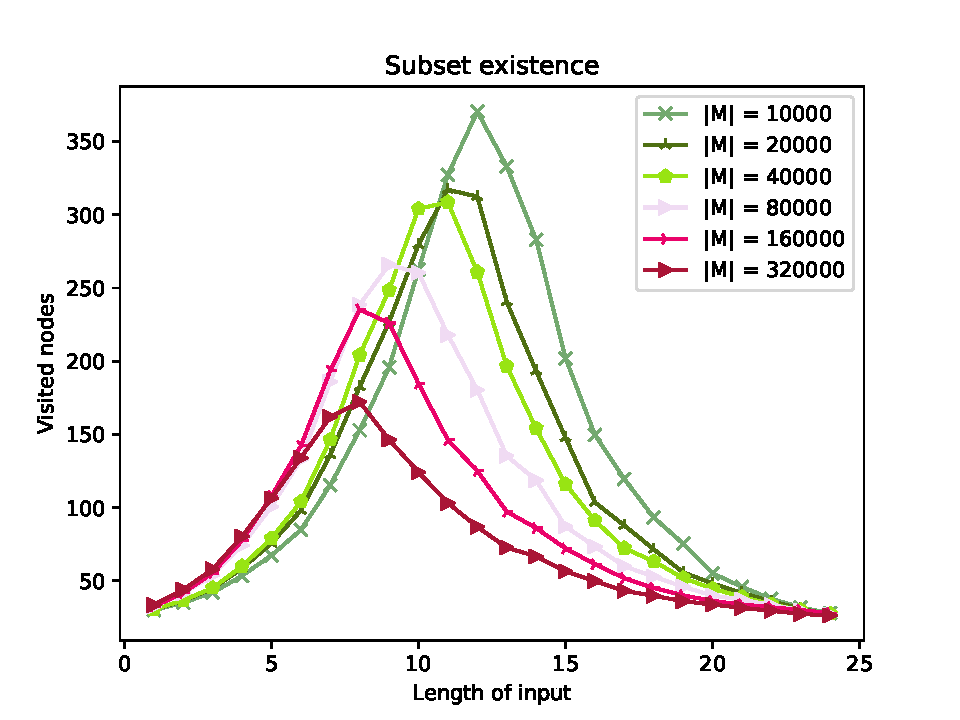
\includegraphics[width=.4\textwidth]{exp1-m1.pdf}
\caption{Experiment 1, submsetExistence function.}
\label{fig:e1m1}
\end{figure}

\begin{figure}
\center
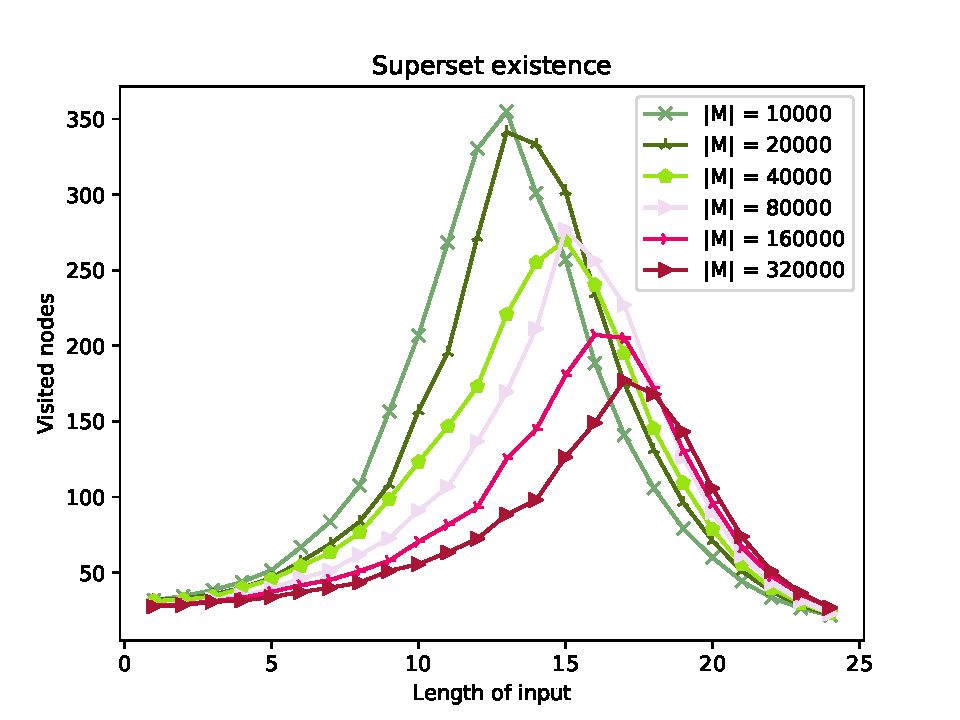
\includegraphics[width=.4\textwidth]{exp1-m2.pdf}
\caption{Experiment 1, supermsetExistence function.}
\label{fig:e1m2}
\end{figure}

\begin{figure}
\center
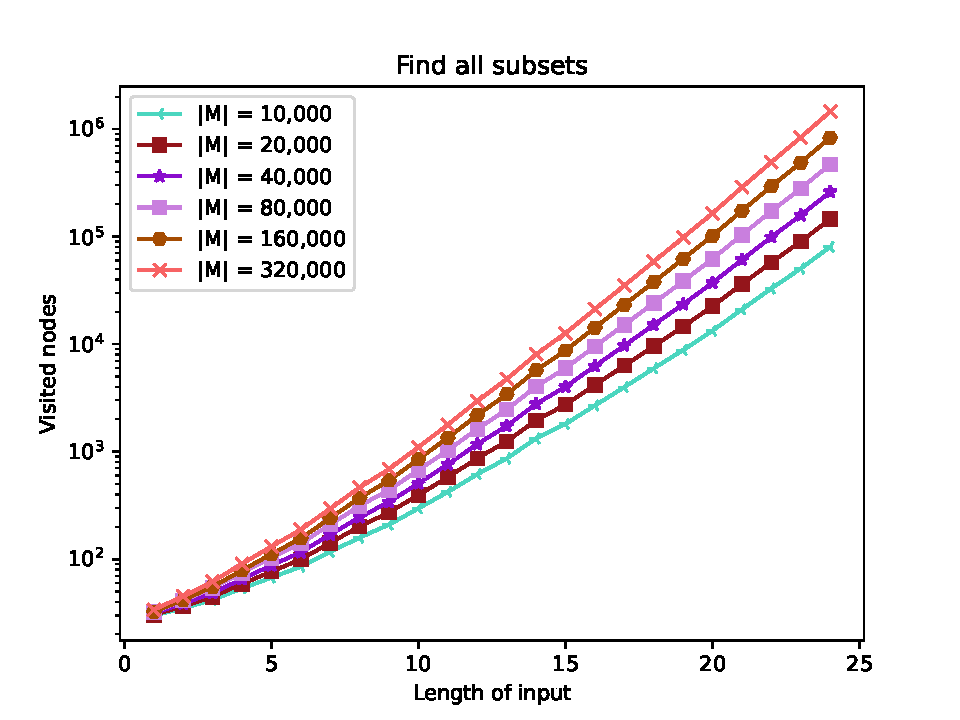
\includegraphics[width=.4\textwidth]{exp1-m3.pdf}
\caption{Experiment 1, getAllSubmsets function.}
\label{fig:e1m3}
\end{figure}

\begin{figure}
\center
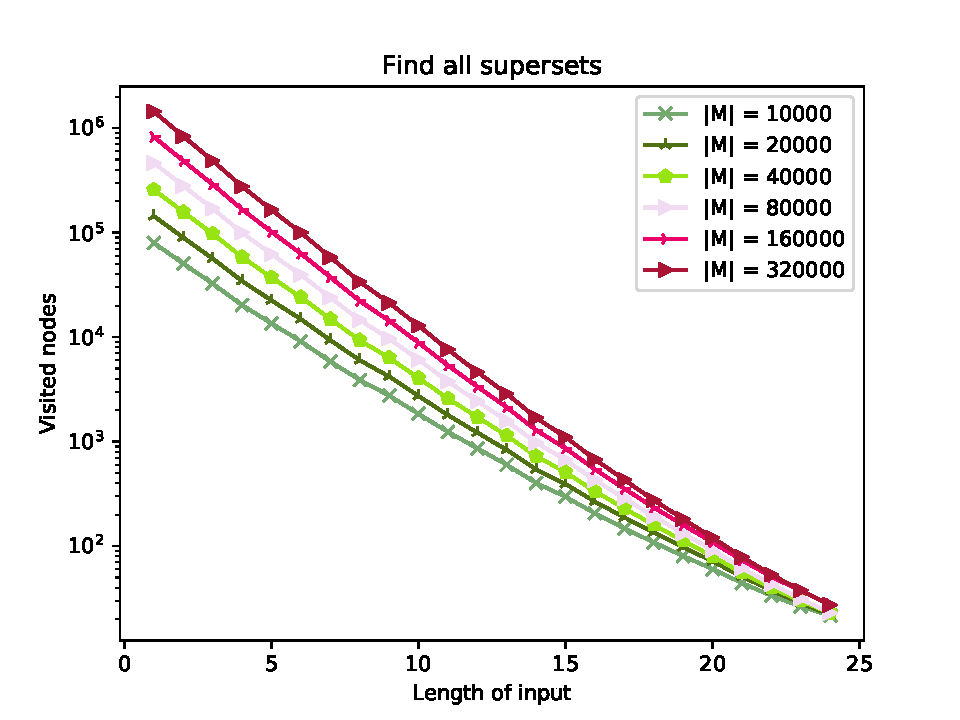
\includegraphics[width=.4\textwidth]{exp1-m4.pdf}
\caption{Experiment 1, getAllSupermsets function.}
\label{fig:e1m4}
\end{figure}

The performance of the functions \textsc{submsetExistence} and 
\textsc{supermsetExistence} increases as the density increases (see figures~\ref{fig:e1m1}
and~\ref{fig:e1m2}). The results are as expected, because the increase of the 
density increases the probability of finding submultiset or supermultiset in 
multiset-trie, which leads to the lower number of visited nodes. 

The maxima are located between 175 and 375 for \textsc{submsetExistence} and 
between 175 and 350 for \textsc{supermsetExistence}. According to those maxima 
we can deduce that at least 7-15 multisets were checked in order to find 
submultiset or supermultiset, which is from $\num{0.02e-3}$ to $\num{1.5e-3}$ of the 
multiset-trie and from $\num{1.9e-7}$ to $\num{4.5e-7}$ of the complete 
multiset-trie.

As the density increases the peaks shift from the center to the left, or to the right, 
for \textsc{submsetExistence} and \textsc{supermsetExistence} respectively. 
The shifts are the consequence of the uniform distribution of sets in $M.$ 
Since every set has the same probability to appear in $M,$ the distribution of set 
sizes in $M$ is normal. Consequently, with increase of the density of the 
multiset-trie the number of sets in $M$ with cardinality $\frac{1}{2}\sigma$ will be 
larger than the number of sets with cardinality $\frac{1}{2}\sigma\pm\epsilon,$ 
for $\frac{1}{2}\sigma > \epsilon > 0.$ So the function \textsc{submsetExistence} 
needs to visit less nodes for test sets of size $\frac{1}{2}\sigma$ than for test 
sets of size $\frac{1}{2}\sigma\pm\epsilon.$ The function decreases the 
multiplicity of some elements (in some cases skips them) in order to find the 
closest subset. Hence, the peak shifts to the left. Oppositely the function 
\textsc{supermsetExistence} increases the multiplicity of some elements 
(in this case adding new elements) in order to find the closest superset. 
Thus, the peak shifts to the right.

Note that despite the peak shifts both functions \textsc{submsetExistence} and 
\textsc{supermsetExistence} have approximately the same worst case performance. 

The performance of the functions \textsc{getAllSubmsets} and \textsc{getAllSupermsets} 
decreases as the density increases (see figures~\ref{fig:e1m3} and~\ref{fig:e1m4}). 
This happens because the number of multisets in multiset-trie increases, which means 
that any multiset in the data structure will have more sub- and supermultisets. 
The maxima for both functions varies from $\num{8.0e4}$ to $\num{1.5e6}$ visited nodes. 
We can notice that local maxima for the functions \textsc{getAllSubmsets} and 
\textsc{getAllSupermsets} differs with respect to the length of input. The 
explanation is very simple. In order to find all submultisets of a small set the 
function has to traverse a small part of multist-trie. As the size of a set 
increases the part of a multiset-trie where all the submultisets of a given set 
are stored also increases. The opposite holds for the function 
\textsc{getAllSupermsets}.


Despite the fact that for a lookup of any set/multiset $\sigma$ nodes must be visited 
in multiset-trie on average case, the data structure has a very similar performance 
results in comparison to the \emph{set-trie} data structure.

\subsection{Experiment 2} \label{s:exp2}
In the Experiment~\hyperref[s:exp2]{2} we demonstrate the performance of 
the unrestricted multiset-trie allowing \emph{multisets} to be inserted into data structure. 
We set $n$ to be 6 and retain $\sigma = 25$ as it was in Experiment~\hyperref[s:exp1]{1}. 
The mapping $\phi$ does not have an influence on results, since the input 
data is generated artificially with uniform distribution. The cardinality of $M$ 
varies from 40000 to 640000 multisets. Thus, the calculated density $d$ varies 
from $\num{1.4e-15}$ to $\num{2.25e-14}.$ The density is much smaller than 
in Experiment~\hyperref[s:exp1]{1}, because now we allow multisets to be stored 
in the data structure and according to the parameters $n$ and $\sigma$ the 
cardinality of $N$ is $6^{25} = \num{2.84e19}.$

\begin{figure}
\center
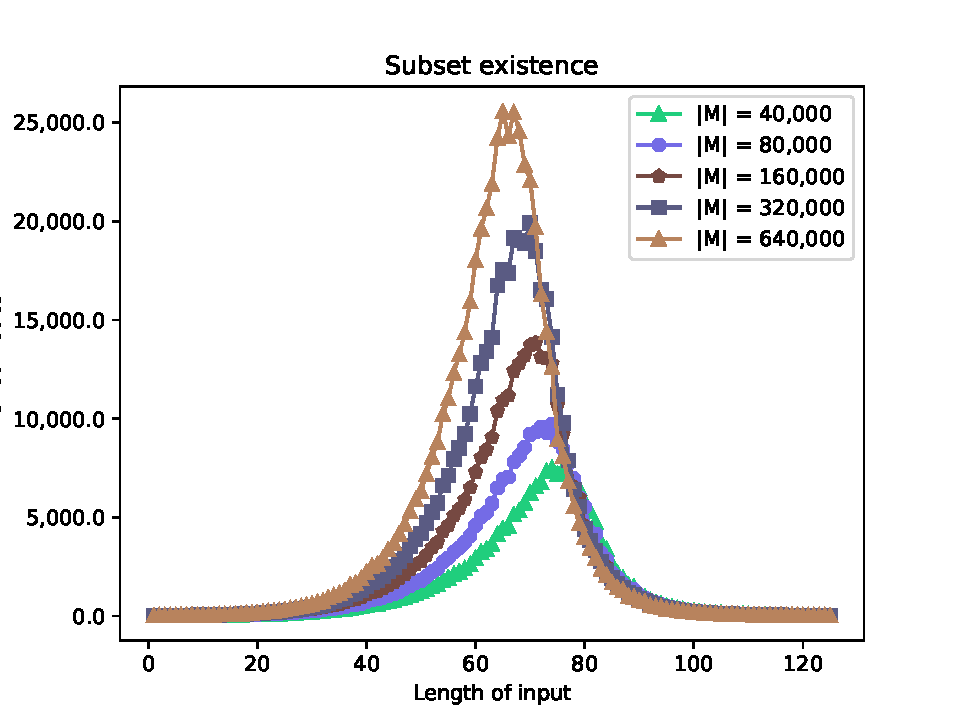
\includegraphics[width=.4\textwidth]{exp2-m1.pdf}
\caption{Experiment 2, submsetExistence function.}
\label{fig:e2m1}
\end{figure}

\begin{figure}
\center
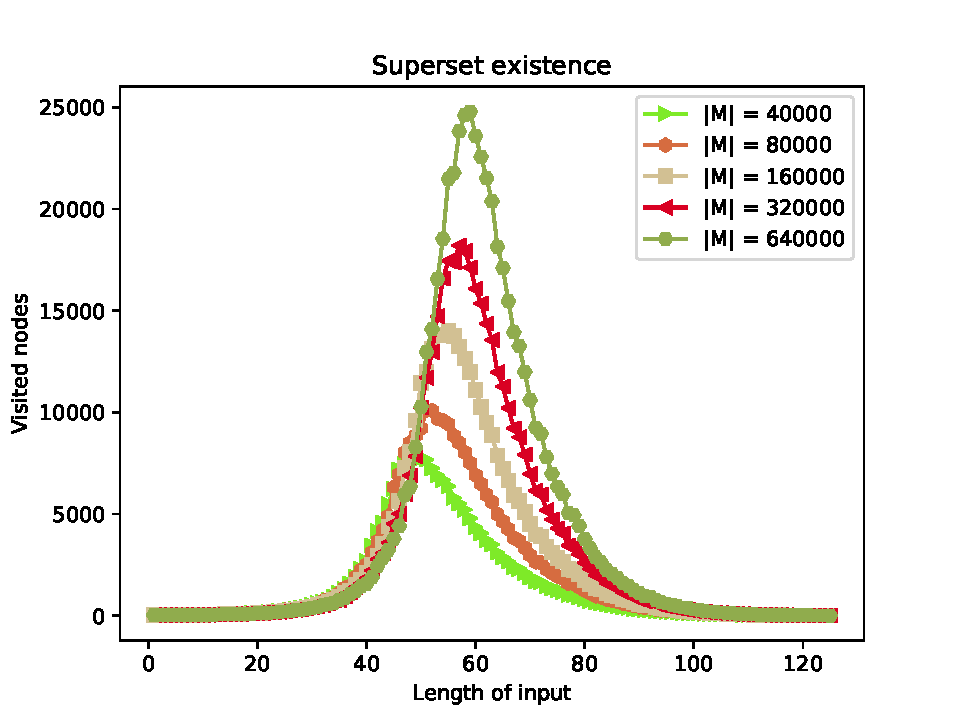
\includegraphics[width=.4\textwidth]{exp2-m2.pdf}
\caption{Experiment 2, supermsetExistence function.}
\label{fig:e2m2}
\end{figure}

\begin{figure}
\center
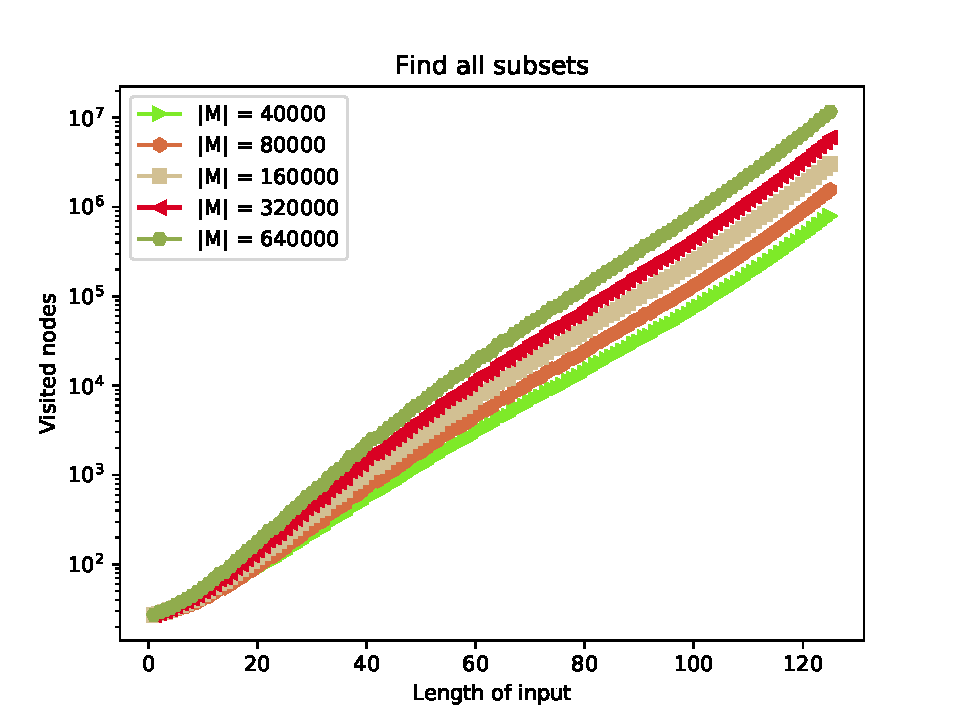
\includegraphics[width=.4\textwidth]{exp2-m3.pdf}
\caption{Experiment 2, getAllSubmsets function.}
\label{fig:e2m3}
\end{figure}

\begin{figure}
\center
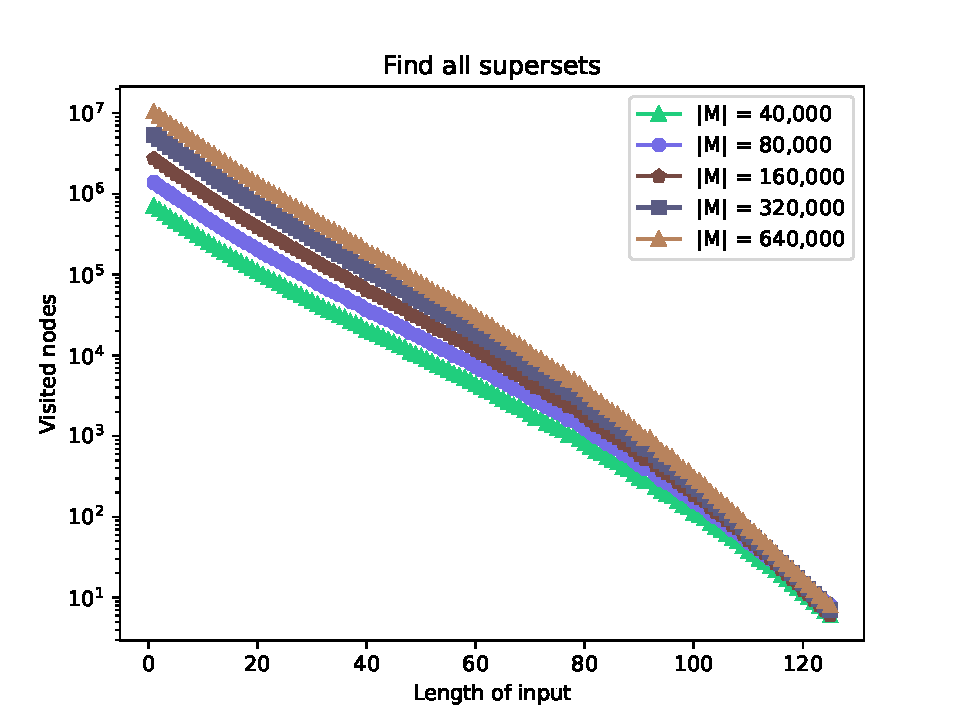
\includegraphics[width=.4\textwidth]{exp2-m4.pdf}
\caption{Experiment 2, getAllSupermsets function.}
\label{fig:e2m4}
\end{figure}

As we can see from the graphs on figures~\ref{fig:e2m1} and~\ref{fig:e2m2}, 
the performance of the functions \textsc{submsetExistence} and 
\textsc{supermsetExistence} becomes worse as the density increases. 
In this case the number $|M|$ is slightly larger than in the 
Experiment~\hyperref[s:exp1]{1}, but the density is very small. Consequently 
multiset-trie become more sparse. Multisets in a sparse multiset-trie differs more, 
which leads to the larger number of visited nodes. 

The maxima for both functions varies from 7500 to 25000 visited nodes. According 
to those maxima at least 300-1000 multisets were checked in order to find 
submultiset or supermultiset, which is from $\num{1.5e-3}$ to $\num{7.5e-3}$ of the entire 
multiset-trie and from $\num{1.1e-17}$ to $\num{3.4e-17}$ of the complete 
multiset-trie. The percentage of visited multisets with respect to $|M|$ is 
larger than in the Experiment~\hyperref[s:exp1]{1}. However, if one would compare 
the percentage of visited multiset with respect to complete multiset-trie, then 
in case of Experiment~\hyperref[s:exp2]{2} it is less by 10 orders than in the 
Experiment~\hyperref[s:exp1]{1}.

The peaks are shifted from the center to the left and right for 
\textsc{submsetExistence} and \textsc{supermsetExistence} respectively. Such a 
behavior was previously observed in the Experiment~\hyperref[s:exp1]{1}. The 
explanation is the same: the input data has uniform distribution, implying that 
the size of multisets in $M$ is normally distributed. Because of the normal 
distribution of size of multisets the shift of the peak occurs as the density increases.

It can be also observed that as in previous Experiment~\hyperref[s:exp1]{1} both 
functions \textsc{submsetExistence} and \textsc{supermsetExistence} have similar 
worst case performance. 

The functions \textsc{getAllSubmsets} and \textsc{getAllSupermsets} decrease 
their performance as the density increases (see figures~\ref{fig:e2m3} 
and~\ref{fig:e2m4}). It happens, because the number of multisets increases as 
the density increases. So there are more nodes have to be visited in order to 
retrieve all sub- or supermultisets of some multiset. The maximum for both functions 
varies from $\num{0.9e5}$ to $\num{1.5e7}$ visited nodes. As it was observed in 
Experiment~\hyperref[s:exp1]{1} the maxima occur at the opposite points. For the 
function \textsc{getAllSubmsets} it will always be at the largest size of multiset, 
which is 125 in our case. Conversely the maximum for the \textsc{getAllSupermsets} 
is at the smallest size of multiset, which is 0 (an empty set).

The results of the Experiment~\hyperref[s:exp1]{1} show that the performance 
of functions \textsc{submsetExistence} and \textsc{supermsetExistence} increases 
as the density increases. However, we observe the opposite behavior in the 
Experiment~\hyperref[s:exp2]{2}. We explain the reason of such a contradiction 
in the next Experiment~\hyperref[s:exp3]{3} 


%\subsection{Experiment 3}
%In this experiment we vary $\sigma$ from 10 up to 70. The maximal degree node 
%$n$ is set to 6 and the input data $|M|$ is set to 640000 multisets. This way 
%we extremly decrease density $d$ as we increase $\sigma.$ 
%The density varies from $1.0\%$ to $\num{2.1e-47}\%.$
%
%\begin{figure}
%\center
%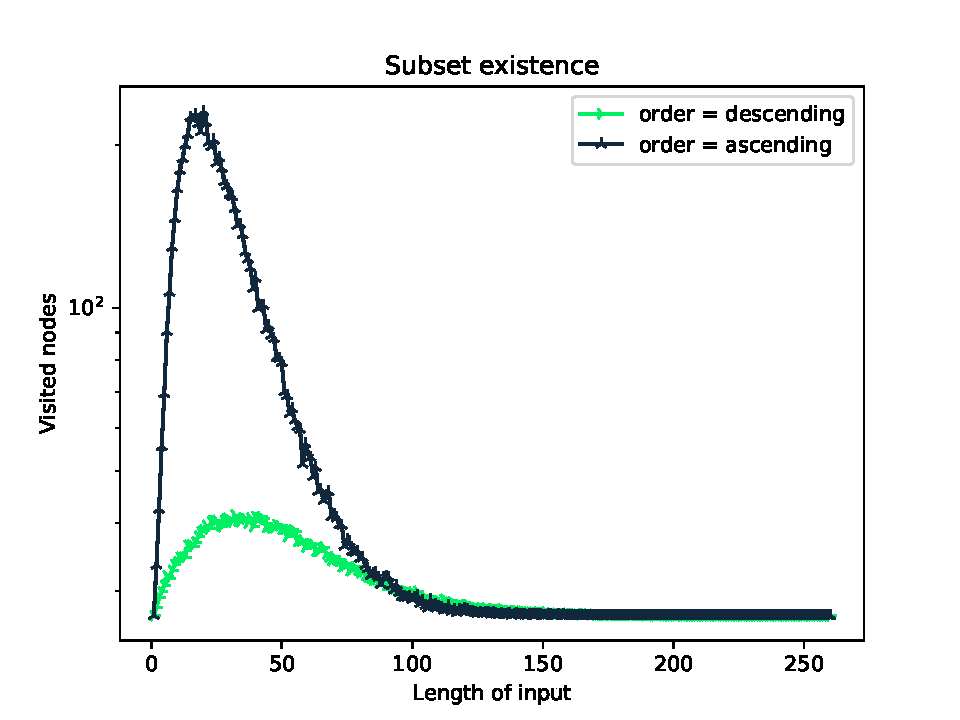
\includegraphics[width=.9\textwidth]{exp3-m1.pdf}
%\caption{Experiment 3, submsetExistence function.}
%\end{figure}
%
%\begin{figure}
%\center
%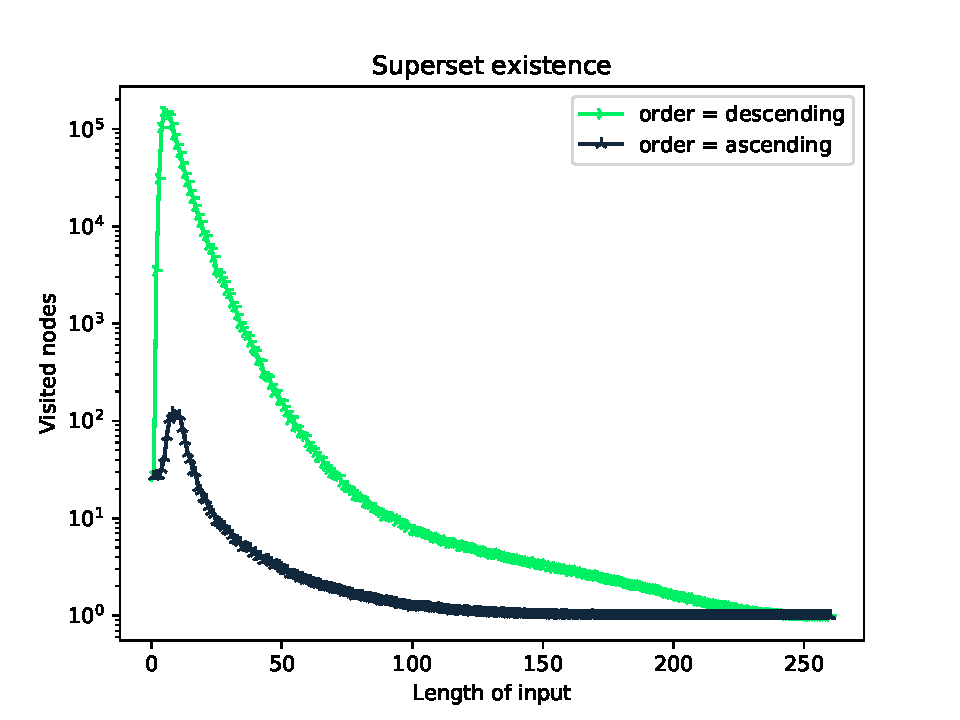
\includegraphics[width=.9\textwidth]{exp3-m2.pdf}
%\caption{Experiment 3, supermsetExistence function.}
%\end{figure}
%
%\begin{figure}
%\center
%\includegraphics[width=.9\textwidth]{exp3-m3.pdf}
%\caption{Experiment 3, getAllSubmsets function.}
%\end{figure}
%
%\begin{figure}
%\center
%\includegraphics[width=.9\textwidth]{exp3-m4.pdf}
%\caption{Experiment 3, getAllSupermsets function.}
%\end{figure}


\subsection{Experiment 3} \label{s:exp3}
The results of the Experiment~\hyperref[s:exp1]{1} and Experiment~\hyperref[s:exp2]{2} 
have shown that as the density of a multiset-trie increases the performance of 
functions \textsc{submsetExistence} and \textsc{supermsetExistence} can both get 
better and worse. The reason of such a behavior is that the dependence of the 
number of visited nodes on density is not a linear function. It is obvious that the 
performance of the mentioned above functions is maximal when multiset-trie is 
complete. As multiset-trie becomes more sparse (the density is small) multisets 
differ more and the number of visited nodes increases. However, when the density 
is high, multisets differ less, so the number of visited nodes decreases. Since 
the dependence of the number of visited nodes on the density of multiset-trie 
is a continuous function on the interval $[0,1],$ there exists a global maximum. 
In other words there exists such a value of density where the number of visited 
nodes is maximal. 

In this experiment, we empirically find the extremum of density for functions 
\textsc{submsetExistence} and \textsc{supermsetExistence}. The parameters 
$\sigma$ and $n$ are set to 12 and 5 respectively. The density varies from 
$\num{1.0e-6}$ to $\num{1.0e-2}.$ The number of visited nodes was chosen to be 
maximal for each value of particular density.

\begin{figure}
\center
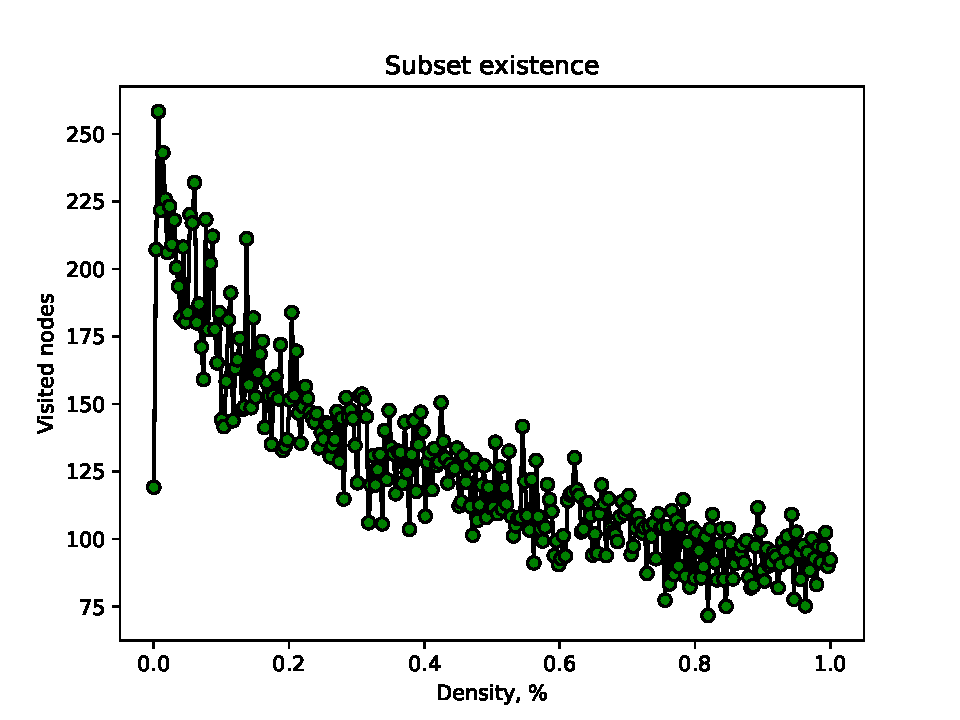
\includegraphics[width=.4\textwidth]{exp4-m1.pdf}
\caption{Experiment 3, submsetExistence function.}
\label{fig:e3m1}
\end{figure}

\begin{figure}
\center
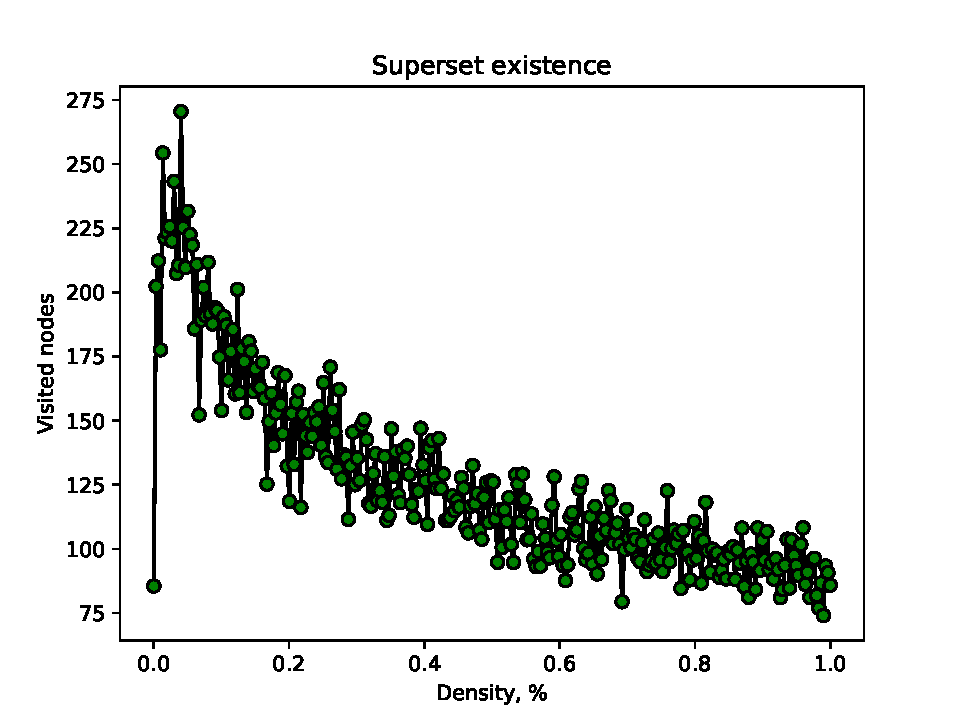
\includegraphics[width=.4\textwidth]{exp4-m2.pdf}
\caption{Experiment 3, supermsetExistence function.}
\label{fig:e3m2}
\end{figure}

As we see on figures~\ref{fig:e3m1} and~\ref{fig:e3m2} both functions 
\textsc{submsetExistence} and \textsc{supermsetExistence} have the maximum 
around $d\approx \num{7.0e-5}.$ The maximum is less than $\num{0.3e-3}$ and 
greater than $\num{1.4e-15},$ which explains the behavior of multiset-trie in 
Experiment~\hyperref[s:exp1]{1} and Experiment~\hyperref[s:exp2]{2}. It is safe 
to say that the maximum may vary depending on parameters $n$ and $\sigma,$ but 
such a maximum always exists. Therefore, we omit the experiments with different 
parameters $n$ and $\sigma.$


\subsection{Experiment 4} \label{s:exp4}
In previous experiments the input was generated artificially with uniform 
distribution, so there was no influence of the mapping function $\phi$ on 
performance of tested functions. This experiment shows the influence of the 
mapping $\phi$ from alphabet $\Sigma$ to a set of consecutive integers. 
We obtain the influence by taking the real world data as an input data. 

The data is taken from English dictionary which contains 235883 different words. 
Those words are mapped to multisets of integers according to the $\phi.$ In 
particular, we are interested in cases when $\phi(\Sigma)$ enumerates 
letters by their relative frequency in English language. We say that $\phi(\Sigma)$ 
maps letters in \emph{ascending order} if the most frequent letter is mapped to 
number $\sigma.$ Conversely, in \emph{descending order} this letter is mapped to 
number $1.$ The size of the alphabet $\sigma$ is set to the size of the English 
alphabet 26. The degree of a node $n$ is set to 10. On average the multiplicity 
of letters is of course less than 10. We choose such a large node degree allowing 
the multiplicity to be up to 10, because the dictionary contains such words. 


\begin{figure}
\center
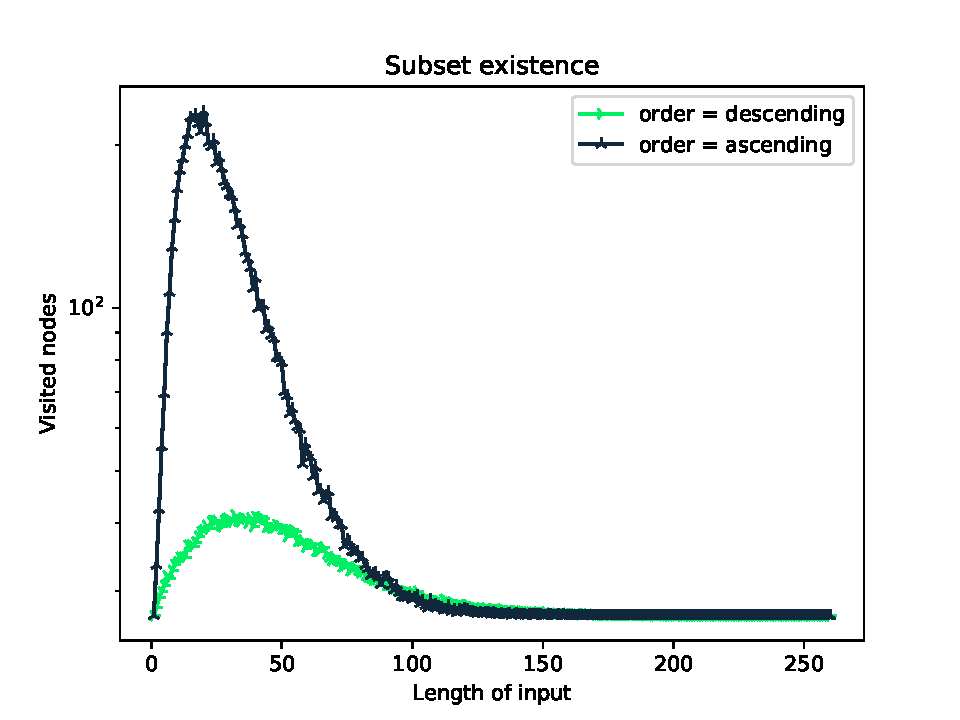
\includegraphics[width=.4\textwidth]{exp3-m1.pdf}
\caption{Experiment 4, submsetExistence function.}
\label{fig:e4m1}
\end{figure}

\begin{figure}
\center
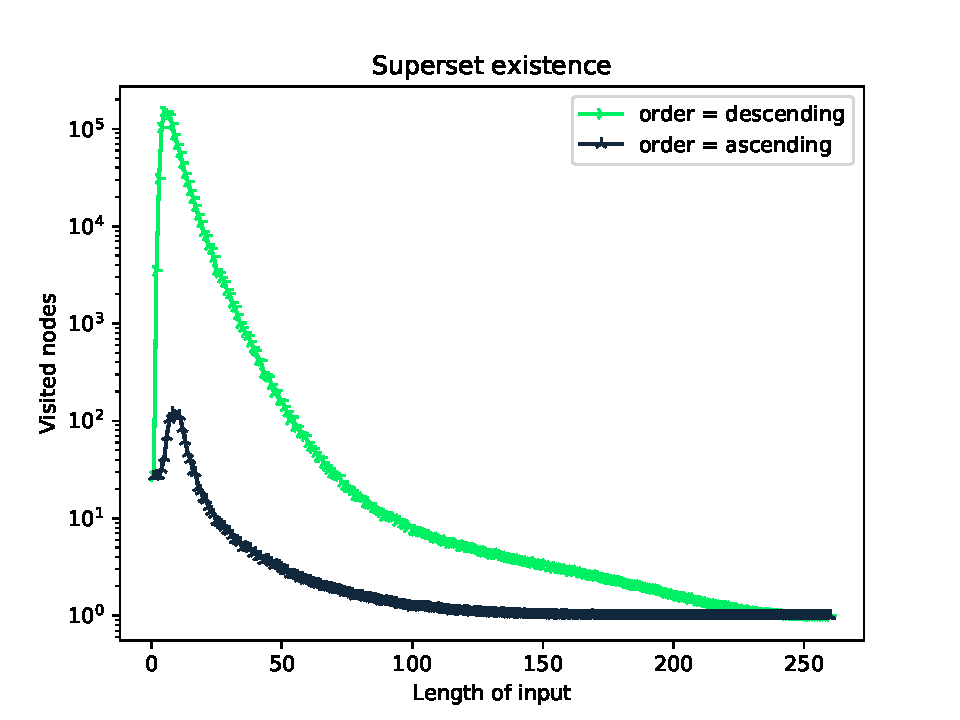
\includegraphics[width=.4\textwidth]{exp3-m2.pdf}
\caption{Experiment 4, supermsetExistence function.}
\label{fig:e4m2}
\end{figure}

%\begin{figure}
%\includegraphics[width=\textwidth]{exp4-m3.pdf}
%\caption{Experiment 4, getAllSubmsets function.}
%\end{figure}
%
%\begin{figure}
%\includegraphics[width=\textwidth]{exp4-m4.pdf}
%\caption{Experiment 4, getAllSupermsets function.}
%\end{figure}

The results on figures~\ref{fig:e4m1} and~\ref{fig:e4m2} are more balanced when 
letters are ordered by frequency in ascending order. The maxima for the functions 
\textsc{submsetExistence} and \textsc{supermsetExistence} are at 250 visited nodes. 

According to the design of the data structure multiset-trie, we can say 
something about multiset only if we try to reach it, i.e. to find the complete 
path that corresponds to a particular multiset. It means that in order to give 
an answer whether some multiset exists or not one have to check the leaf level in 
multiset-trie. 

Letters that have the least frequencies are now located at the top of 
multiset-trie according to ascending order of letters by frequency. This means 
that the search becomes narrower, because a lot of invalid paths will be 
discarded on top most levels. Thus, multiset-trie can be traversed faster.

As you may have noticed the functions \textsc{getAllSubmsets} and 
\textsc{getAllSupermsets} were not tested in this experiment. Those functions 
are not affected by variations of the mapping $\phi,$ because for any multiset 
they retrieve all sub/supermultisets. This means that the number of visited 
nodes will not be changed as $\phi$ varies.

\subsection{Experiment 5} \label{s:exp5}
In this experiment we demonstrate the performance of multiset-trie data structure 
compared to B+ tree based inverted index. The data structure is also implemented 
in~\CC{ to} avoid any optimization or degradation of performance caused by different 
programming language implementation.

During tests both data structures used the same interface for benchmark that operates 
with files as its input and output. Each data structure was loaded with the same input data 
and was queried with the same test data. The input and test data were generated artificially 
according to parameters $\sigma$ and $n.$ The combinations of parameters is as follows in the 
Table~\ref{t:benchmark}.

\begin{table}[h]
\center
\begin{tabular}{|c|c|}
\hline
$\sigma$ & $n$ \\
\hline
5		& 1\\
\hline
30	& 1 \\
\hline
5		& 3 \\
\hline
15	& 3 \\
\hline
30	& 3 \\
\hline
10	& 10 \\
\hline
\end{tabular}
\caption{Configuration of $\sigma$ and $n$ in benchmark.}
\label{t:benchmark}
\end{table}

We tested all the three types of query on all of the configurations from the Table~\ref{t:benchmark} which 
results in 18 experiments total, i.e. 6 experiments per query type. In each of the experiment we measured an 
average time consumed by the data structure to process the query. 

The results of the exact search, submultiset search and supermultiset search experiments are shown in the tables 
Table~\ref{t:res_ex}, Table~\ref{t:res_sub} and Table~\ref{t:res_sup} respectively .

\begin{table}[h]
\center
\begin{tabular}{|c|c|c|c|}
\hline
$\sigma$ & $n$ & Multiset-trie ($\mu s$) & Inverted index ($\mu s$) \\
\hline
5		& 1 & 3.45 & 17782.35\\
\hline
30	& 1 & 4.18 & 24865.93\\
\hline
5		& 3 & 2.20 & 1508.81\\
\hline
15	& 3 & 4.39 & 2146.36\\
\hline
30	& 3 & 10.67 & 3639.97\\
\hline
10	& 10 & 6.93 & 384.05\\
\hline
\end{tabular}
\caption{Exact search.}
\label{t:res_ex}
\end{table}

\begin{table}[h]
\center
\begin{tabular}{|c|c|c|c|}
\hline
$\sigma$ & $n$ & Multiset-trie ($\mu s$) & Inverted index ($\mu s$) \\
\hline
5		& 1			& 8.96 & 73500.84\\
\hline
30	& 1			& 17.33 & 547572.74\\
\hline
5		& 3			& 117.95 & 162360.43\\
\hline
15	& 3			& 20.74 & 443321.39\\
\hline
30	& 3 		& 23.75 & 947706.14\\
\hline
10	& 10		& 55.59 & 466022.68\\
\hline
\end{tabular}
\caption{Submultiset search.}
\label{t:res_sub}
\end{table}

\begin{table}[h]
\center
\begin{tabular}{|c|c|c|c|}
\hline
$\sigma$ & $n$ & Multiset-trie ($\mu s$) & Inverted index ($\mu s$)\\
\hline
5		& 1 		& 10.63 & 63073.86\\
\hline
30	& 1 		& 14.65 & 449251.68\\
\hline
5		& 3 		& 171.04 & 163256.77\\
\hline
15	& 3 		& 43.42 & 425733.80\\
\hline
30	& 3 		& 22.06 & 729831.34\\
\hline
10	& 10 	& 58.32 & 373784.81\\
\hline
\end{tabular}
\caption{Supermultiset search.}
\label{t:res_sup}
\end{table}

We can see that multiset-trie outperforms inverted index in all of the experiments by up to 4 orders of magnitude. 
In exact search multiset-trie has to traverse only up to $\sigma+1$ nodes in order to get query result. It is seen 
from results that with increase of $\sigma$ the processing time for multiset-tire also increases. Interestingly, the 
multiplicity also affects the time of processing, however, this happens passively. Multiplicity or degree of a node $n$ 
defines what multisets can be stored in multiset-trie. Thus, it affects the structure and density of the multiset-trie.

As for the inverted index, it must fetch all the postings according to each element in a test multiset and then intersect 
the results in order to answer the query. This is a more time consuming operation than a simple tree traversal, which we 
can see from results. Postings are of course filtered on-the-fly to reduce the cost of intersection, however these are still 
additional operations to be performed. Note, that inverted file will also access at most $\sigma$ postings during search, 
but in addition to access some extra processing is required.

The submultiset and supermultiset basically do not change to much in the case of inverted file, because the algorithm consists 
of the same steps: the postings are fetched according to elements of the test multiset, then they are filtered on-the-fly 
according to the query type, and at the end the postings either has to be united or intersected. So, besides a traversal of at most 
$\sigma$ keys of the index additional processing is required. Note, that every key is mapped to a list of postings which 
can be large as index grows.

In the case of multiset-trie only a traversal of the tree is required which is much faster than processing of postings as we can 
see from results. In the worst case the whole tree is traversed, but so is for inverted file.